\documentclass{article}
\usepackage{graphicx}
\usepackage{fullpage}
\usepackage{amsmath}

\title{Übungsblatt 10}
\author{Tobias Baake (247074), Dylan Ellinger (247316), Nikiforos Tompoulidis (247714)}
\begin{document}
\maketitle

\section{Cohen-Sutherland}
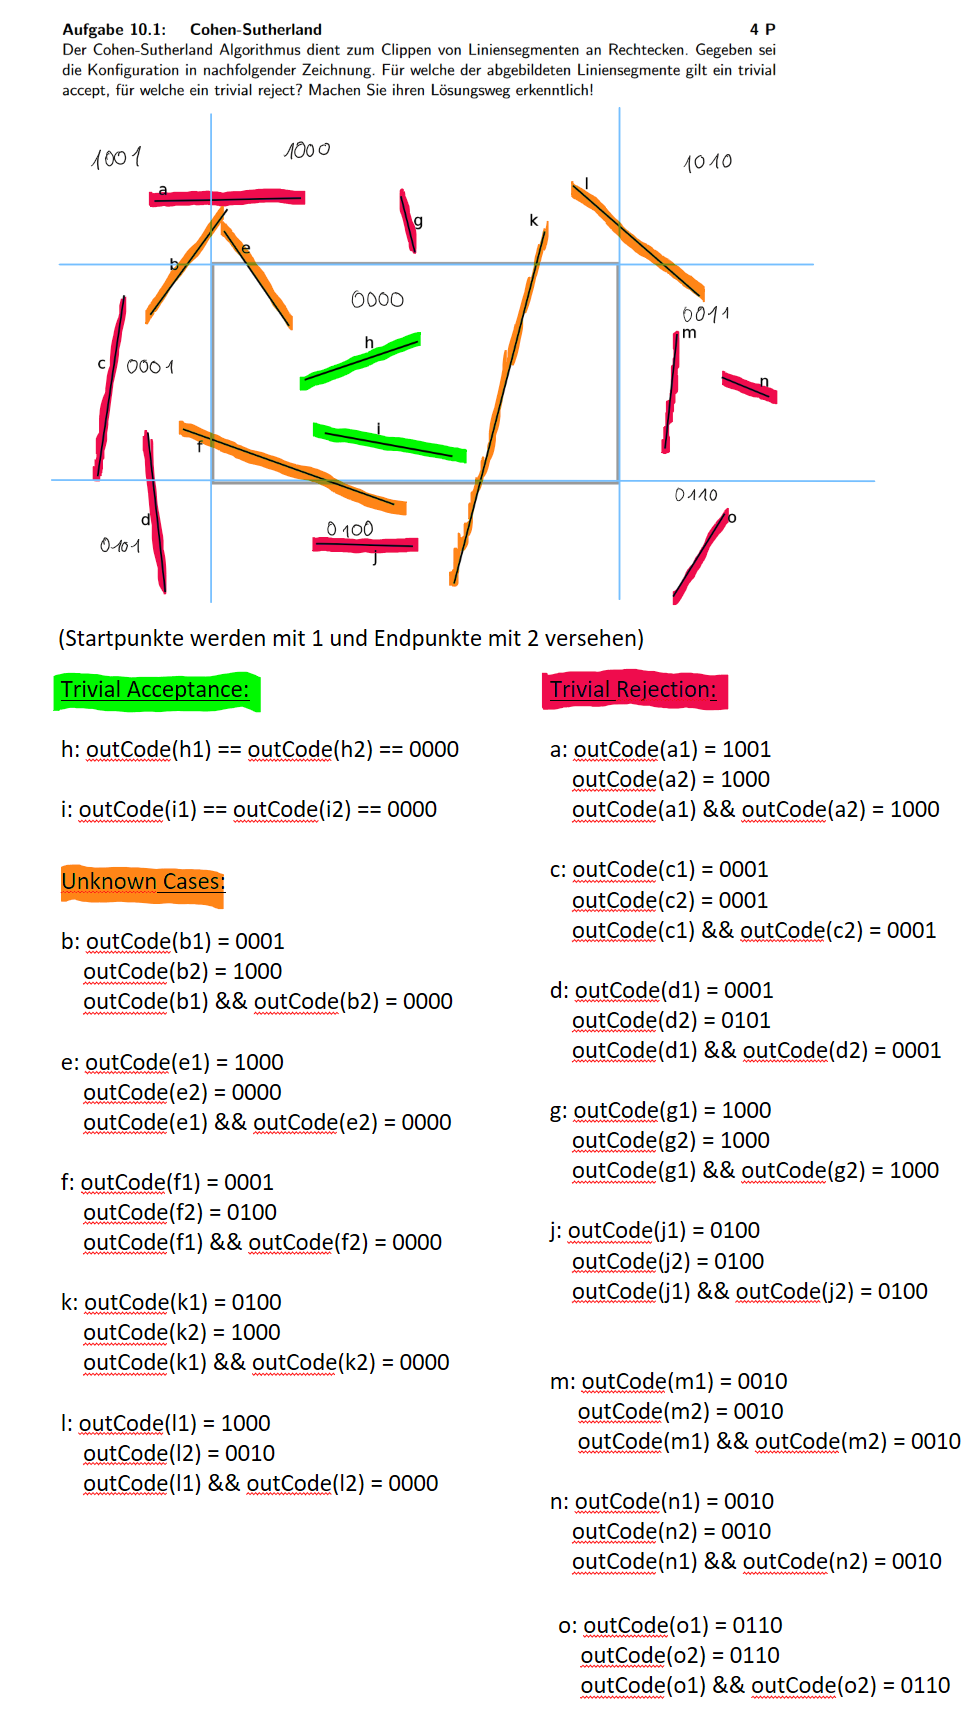
\includegraphics[width=370pt]{./files/Übung10.1.png}

\section{Clipping: Algorithmen}
\subsection*{a)}
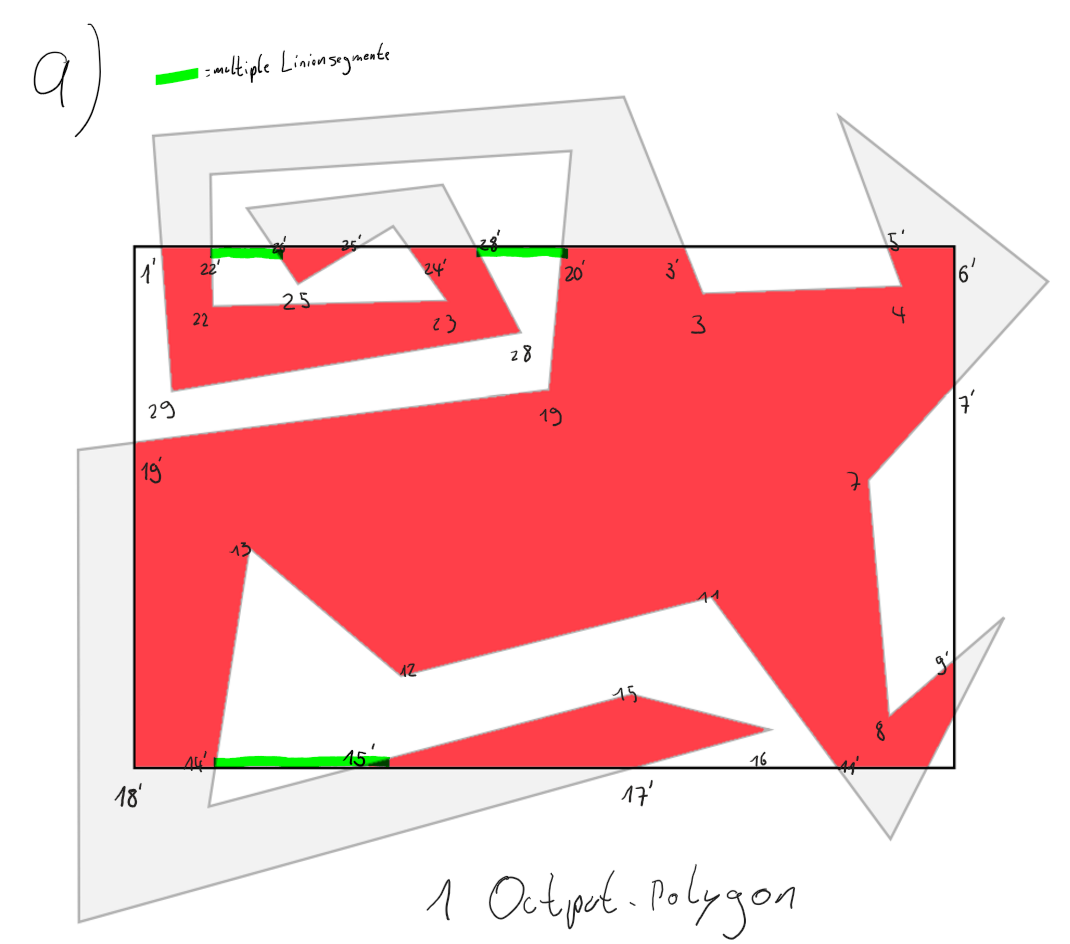
\includegraphics[width=400pt]{./files/Übung10.2a.png}

\subsection*{b)}
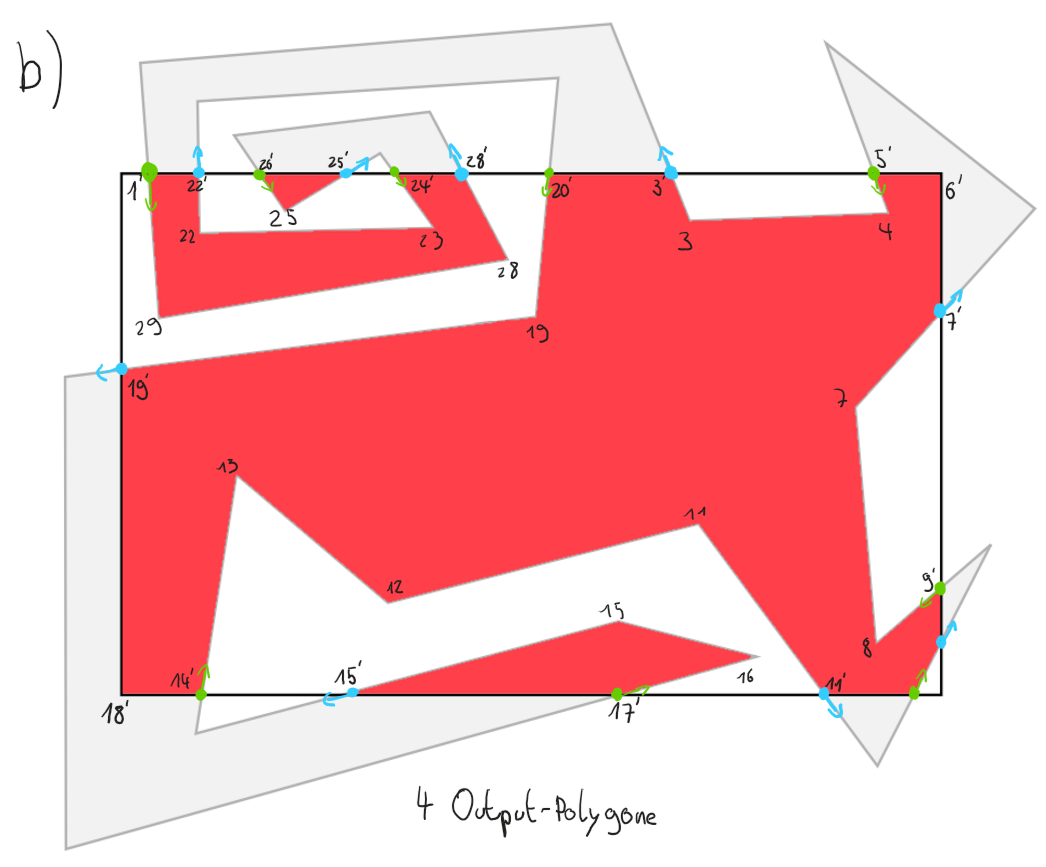
\includegraphics[width=400pt]{./files/Übung10.2b.png}

\section{Clipping}

Betrachten Sie das Clippen eines konvexen Polygons mit n Ecken an einem Rechteck

\subsection*{a) maximale Anzahl von Ecken im geklippten Polygon}
n, weil beim klippen, Punkte außerhalb des Rechtecks (Bildschirm) entfernt werden, jedoch keine neuen hinzugefügt werden. \textbf{Ausnahme/Sonderfall:} wenn nur ein Punkt außerhalb liegt, werden am Rand des Rechtecks durch das Clipping 2 Punkte erzeugt. Somit liegt die maximale anzahl bei \underline{n + 1}.

\subsection*{b) minimale Anzahl von Ecken im geklippten Polygon}
3, wenn wenn genau ein Punkt innerhalb des Rechtecks liegt, spannt dieser ein Dreieck (mit den Seitenkanten des Rechtecks) auf. Wenn alle Punkte außerhalb des Rechtecks liegen ist die Anzahl der Punkte 0 oder wenn nur ein Punkt genau auf einer Kante von den Rechteck liegt, das ist die Anzahl 1.
Das Ergebnis kann man also auf 1 festlegen, der Sonderfall, wo genau eine Ecke des Polygons auf der Seitenkante des Rechtecks liegt.
\\
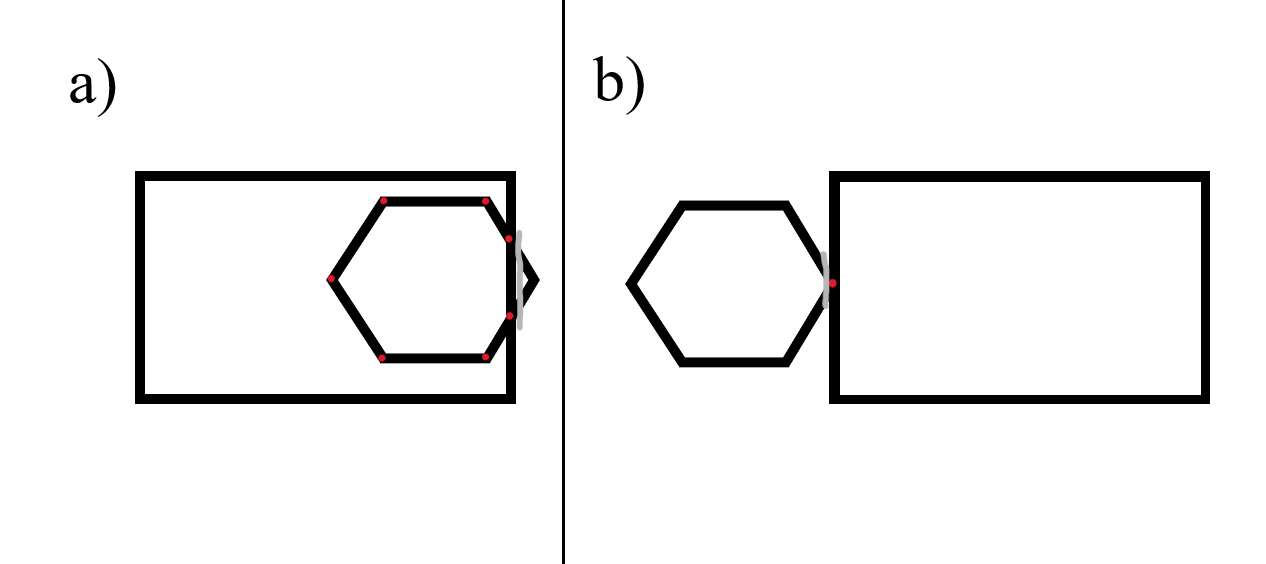
\includegraphics[width=400pt]{./files/Übung10.3.png}
\\
Punkte in Rot liegen innerhalb oder auf des/dem Rechtecks.

\section{Implizite Geraden}

Implizite Form einer Geraden: $ax + by +c = 0$

\subsection*{a)}
$a_1 = (1,2)^T, a_2 = (5,3)^T$

LGS: (mit c = 1)
\begin{align*}
    I \ \ \ & 1x + 5y + 1 = 0 \\
    II \ \ \ & 2x + 3y + 1 = 0 \\
    I \cdot (-2) \ \ \ & -2x - 10y - 2 = 0\\
    II \ \ \ & \underline{ 2x + 3y + 1= 0} \\
    III \ \ \ & -7y - 1 = 0 \\
    \ \ \ \rightarrow & \ \ \ \underline{y = -\frac{1}{7}} \\
\end{align*}
$y = -\frac{1}{7}$ in $I$
\begin{align*}
    x + 5(-\frac{1}{7}) + 1 = 0 \\
    x - \frac{5}{7} + 1 = 0 \\
    x = \frac{5}{7} - 1 \\
    x = \frac{5}{7} - \frac{7}{7} \\
    \underline{x = -\frac{2}{7}} \\
\end{align*}
\textbf{Geradengleichung:} $\underline{\underline{-\frac{2}{7}x + \frac{1}{7}y + 1= 0}}$

\subsection*{b)}
$b_1 = (-2,1)^T, b_2 = (6,-1)^T$

LGS: (mit c = 1)
\begin{align*}
    I \ \ \ & -2x + 6y + 1 = 0 \\
    II \ \ \ & 1x - 1y + 1 = 0 \\
    I  \ \ \ & -2x + 6y + 1 = 0\\
    II \cdot (2)\ \ \ & \underline{ 2x - 2y + 2= 0} \\
    III \ \ \ & 4y + 3 = 0 \\
    \ \ \ \rightarrow & \ \ \ \underline{y = \frac{3}{4}} \\
\end{align*}
$y = -\frac{3}{4}$ in $II$
\begin{align*}
    x + 1(\frac{3}{4}) + 1 = 0 \\
    x + \frac{7}{4} = 0 \\
    \underline{x = -\frac{7}{4}} \\
\end{align*}
\textbf{Geradengleichung:} $\underline{\underline{-\frac{7}{4}x + \frac{3}{4}y + 1 = 0}}$

\subsection*{c)}
$c_1 = (3,4)^T, c_2 = (3,-2)^T$

LGS: (mit c = 1)
\begin{align*}
    I \ \ \ & 3x + 3y + 1 = 0 \\
    II \ \ \ & 4x - 2y + 1 = 0 \\
    I \cdot (-4) \ \ \ & -12x - 12y - 4 = 0\\
    II \cdot 3 \ \ \ & \underline{ 12x - 6y + 3= 0} \\
    III \ \ \ & -18y - 3 = 0 \\
    \ \ \ \rightarrow & \ \ \ \underline{y = -\frac{3}{18}} \\
\end{align*}
$y = -\frac{3}{18}$ in $I$
\begin{align*}
    3x + 3(-\frac{3}{18}) + 1 = 0 \\
    3x - \frac{3}{2} = 0 \\
    3x = \frac{3}{2}\\
    3x = \frac{1}{2}\\
    \underline{x = \frac{1}{2}} \\
\end{align*}
\textbf{Geradengleichung:} $\underline{\underline{-\frac{3}{18}x - \frac{1}{2}y + 1 = 0}}$

\subsection*{d)}
$d_1 = (0,1)^T, d_2 = (-1,0)^T$

LGS: (mit c = 1)

\begin{align*}
    I \ \ \ & 0x + 1y + 1 = 0 & \underline{\rightarrow y = -1} \\
    II \ \ \ & -1x + 0y + 1 = 0 & \underline{\rightarrow x = 1} \\
\end{align*}

\textbf{Geradengleichung:} $\underline{\underline{1x - 1y + 1 = 0}}$
\end{document}